\documentclass{article}

% Packages for code listing and syntax highlighting
\usepackage{listings}
\usepackage{xcolor}
\usepackage[margin=3cm]{geometry} % Adjust the margin value as desired
\usepackage{setspace}
\usepackage{tikz}
\usepackage{graphicx}
\usepackage{float}
\usepackage{textcomp}
\usepackage{multicol}
\usepackage{enumitem}

\onehalfspacing

% Define the color theme
\definecolor{codebackground}{RGB}{242, 242, 242}
\definecolor{codekeyword}{RGB}{0, 0, 255}
\definecolor{codecomment}{RGB}{63, 127, 95}
\definecolor{codestring}{RGB}{163, 21, 21}

% Code listing style for all languages
\lstdefinestyle{mystyle}{
    backgroundcolor=\color{codebackground},
    basicstyle=\footnotesize\ttfamily,
    keywordstyle=\color{codekeyword}\bfseries,
    commentstyle=\color{codecomment}\itshape,
    stringstyle=\color{codestring},
    numbers=left,
    numberstyle=\tiny\color{codecomment},
    stepnumber=1,
    numbersep=8pt,
    showstringspaces=false,
    breaklines=true,
    frame=single,
    frameround=none,
    framesep=5pt,
    rulecolor=\color{codebackground},
    tabsize=4,
    captionpos=b,
    xleftmargin=15pt,
    xrightmargin=15pt
}

% Set the default style for code listings
\lstset{style=mystyle}

% Additional packages and settings for math typesetting
\usepackage{amsmath}
\usepackage{amssymb}
\usepackage{bm}

% Define your document content
\begin{document}

\title{Encoding Integers in Binary Logic}
\author{Abyan Majid}
\date{July 5, 2023}
\maketitle

\begin{center}
    \fbox{For the sake of simplicity, I will only be encoding 8-bit integers in this note.} \\
    Of course, the encoding methods in this note is also applicable to higher-bit integers.
\end{center}

\section{Size \& magnitude notation}
In size \& magnitude notation, the leftmost bit represents the sign ("0" means positive, "1" means negative), meanwhile the remaining bits represents the magnitude of the integer.
\begin{center}
    \fbox{$\square$}\fbox{$\square\square\square\square\square\square\square$}
\end{center}

\begin{center}
    \noindent Suppose we want to translate the integer "-25" to binary.
\end{center}

\begin{enumerate}
    \item First, we get the magnitude of -25 (which is just the binary of its natural, or $\lvert -25 \rvert$). \\
    \fbox{$\square$}\fbox{0011001}
    \item Second, Make the leftmost bit = 1. \\
    \fbox{1}\fbox{0011001} \\
\end{enumerate}

\vspace{-\baselineskip}

\begin{center}
    So, the 8-bit binary of "-25" is \fbox{10011001}
\end{center}

\noindent \hrulefill \\
\subsubsection{Two encoding of 0}
\noindent This method is much more intuitive than 2s complement, but it has an undesirable property which is that zero has two possible encodings which are:
\begin{itemize}
    \item $000...0$
    \item $100...0$
\end{itemize}

\noindent This is because 0 is neither positive or negative.\\

\begin{center}
    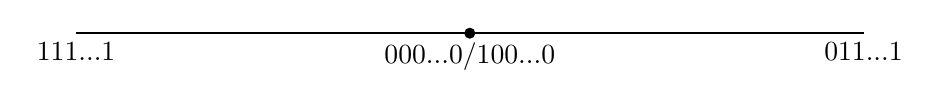
\begin{tikzpicture}
        \draw[-, line width=0.75pt] (-5,0) -- (5,0);
        \coordinate (a) at (0,0);
        \fill (a) circle (2pt) node[below] {$000...0/100...0$};
        \node[below] at (-5, 0) {$111...1$};
        \node[below] at (5, 0) {$011...1$};
    \end{tikzpicture}
\end{center}

\vspace{\baselineskip}
\noindent And that is why this method is less desirable. In all circumstances, you should encode integers in 2s complement notation.

\section{2s complement notation (Preferred Method)}

In 2s complement notation, we discard the undesirable property that 0 has two encodings by letting 0 be equal to only $000...0$ and inverting the bits for every negative integer.

\vspace{\baselineskip}
\begin{center}
    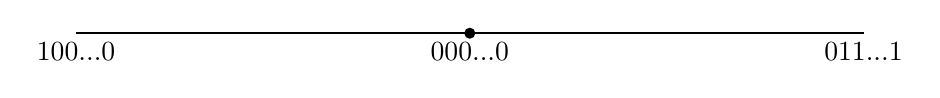
\begin{tikzpicture}
        \draw[-, line width=0.75pt] (-5,0) -- (5,0);
        \coordinate (a) at (0,0);
        \fill (a) circle (2pt) node[below] {$000...0$};
        \node[below] at (-5, 0) {$100...0$};
        \node[below] at (5, 0) {$011...1$};
    \end{tikzpicture}
\end{center}

\noindent To translate a positive integer, you treat it like a natural and get the binary. On the other hand, to translate  a negative integer, say "$-25$", you follow these steps:
\begin{enumerate}
    \item Get the binary representation of the integer \\
    \fbox{00011001}
    \item Invert all the bits to get the 1s complement (so you turn 0s to 1s, and 1s to 0s) \\
    $\fbox{00011001}\rightarrow\fbox{11100110}$ (this is the 1s complement)
    \item Add 1 to the 1s complement \\
        \[
        \begin{array}{r}
            11100110 \\
        +  1 \\
        \hline
            11100111 \\
        \end{array}
        \]        
\end{enumerate}

\begin{center}
    So, the 8-bit binary of "$-25$" is \fbox{11100111}.
\end{center}

\noindent Furthermore, this method also allows us to consistently perform basic arithmetic between binary numbers. Suppose we want to add 10 to -25,
\[
    \begin{array}{r}
        -25 \\
    +  10 \\
    \hline
        -15 \\
    \end{array}
\]

\begin{center}
    But in binary logic. So, given that the 8-bit binary of 10 is 00001010, we have:
\end{center}
\[
    \begin{array}{r}
        11100111 \\
    +  00001010 \\
    \hline
        11110001 \\
    \end{array}
\]
\begin{center}
    The 8-bit binary of $-15$ is indeed $11110001$, so this proves that the 2s complement notation allows for arithmetic operations between binary numbers.
\end{center}

\end{document}